% to choose your degree
% please un-comment just one of the following
\documentclass[bsc,logo,frontabs,twoside,singlespacing,normalheadings,parskip]{infthesis}     % for BSc, BEng etc.
% \documentclass[minf,frontabs,twoside,singlespacing,parskip]{infthesis}  % for MInf


% FONT COMMANDS
\usepackage{fontspec}
\setmainfont[Mapping=tex-text,Numbers=OldStyle]{fbb}
\setsansfont[Mapping=tex-text,Numbers=OldStyle,Scale=MatchLowercase]{Gill Sans}
\setmonofont[Mapping=tex-text,Scale=MatchLowercase]{Inconsolata}


% DISPLAY TODOS
% \usepackage[disable]{todonotes}
\usepackage[draft,bordercolor=white,backgroundcolor=yellow!60,linecolor=black,colorinlistoftodos]{todonotes}


% MAKE SURE TODOS ARE INLINE
\let\Oldtodo\todo
\renewcommand{\todo}[1]{\Oldtodo[inline]{#1}}


% ENSURE CHAPTERS WORK IN PDF VIEWERS
\usepackage[]{hyperref}
\hypersetup{
    pdftitle={Storm on Multi-core},
    pdfauthor={Mark Nemec},
    %pdfsubject={Your subject here},
    %pdfkeywords={keyword1, keyword2},
    bookmarksnumbered=true,
    bookmarksopen=true,
    bookmarksopenlevel=1,
    %colorlinks=true,
    pdfstartview=Fit,
    pdfpagemode=UseOutlines,
    pdfpagelayout=TwoPageRight
}

\begin{document}

\title{Storm on Multi-core}

\author{Mark Nemec}

% to choose your course
% please un-comment just one of the following
% \course{Artificial Intelligence and Computer Science}
%\course{Artificial Intelligence and Software Engineering}
%\course{Artificial Intelligence and Mathematics}
%\course{Artificial Intelligence and Psychology }
%\course{Artificial Intelligence with Psychology }
%\course{Linguistics and Artificial Intelligence}
\course{Computer Science}
%\course{Software Engineering}
%\course{Computer Science and Electronics}
%\course{Electronics and Software Engineering}
%\course{Computer Science and Management Science}
%\course{Computer Science and Mathematics}
%\course{Computer Science and Physics}
%\course{Computer Science and Statistics}

% to choose your report type
% please un-comment just one of the following
%\project{Undergraduate Dissertation} % CS&E, E&SE, AI&L
%\project{Undergraduate Thesis} % AI%Psy
\project{4th Year Project Report}

\date{\today}

\abstract{
This is an example of {\tt infthesis} style.
The file {\tt skeleton.tex} generates this document and can be
used to get a ``skeleton'' for your thesis.
The abstract should summarise your report and fit in the space on the
first page.
%
You may, of course, use any other software to write your report,
as long as you follow the same style. That means: producing a title
page as given here, and including a table of contents and bibliography.
}

\maketitle

\section*{Acknowledgements}
Acknowledgements go here.

\tableofcontents

\pagenumbering{arabic}


%%%%%%%%%%%%%%%%%%%%%%%%%%%%%%%%%%%%%%%%%%%%%
%%
%%				INTRODUCTION
%%
%%%%%%%%%%%%%%%%%%%%%%%%%%%%%%%%%%%%%%%%%%%%%


\chapter{Introduction}

In recent years, there has been an explosion of cloud computing software. After Google published their paper on MapReduce \cite{Anonymous:Jj3E6x7v}, many new open-source frameworks for distributed computation have emerged, most notably Apache Hadoop for batch processing and Apache Storm for real-time data stream processing.

The main idea of these frameworks is to split the work that needs to be carried out and distribute it across multiple nodes of a cluster. Commercial companies and researchers have been able to utilise these frameworks and create distributed systems \cite{5billion-sessions} which can accomplish things that would not be possible on a single computer. This has mostly been allowed by the low price of commodity hardware and good horizontal scaling properties.

% TODO: Here talk about What this paper is about !
% TODO: Maybe mention the Hadoop multi-core paper
% TODO: Maybe a section - move main idea here?
This project is about taking the ideas from the distributed system Apache Storm and applying them in the context of multi-core machines instead of clusters.

%% TODO: After that comes Motivation which explains why it's a good idea!
\section{Motivation}

While the cost of a commodity hardware cluster might be lower than the price of a single computer with equal power there are certain limitations:

\begin{itemize}

\item The nodes of a cluster communicate through network. This limits the speed of communication between processes that live on different nodes.

\item Distributed systems waste resources by replicating data to ensure reliability.

% TODO: Maybe mention renting vs owning here
\item Running a distributed computation on commodity hardware usually requires a data centre or renting out instances on cloud computing services such as Amazon EC2 or Rackspace. This is not ideal for some use cases which require full control over the system or a heightened level of security. 

\end{itemize}

On the other hand, even though Moore’s law still holds true, processor makers now favour increasing the number of cores in CPU chips to increasing their frequency. This trend implies that the “free lunch” of getting better software performance by upgrading the processor is over and programmers now have to design systems with parallel architectures in mind. However, there are some limitations to this as well:

\begin{itemize}

\item It is generally believed that writing parallel software is hard. The traditional techniques of message passing and parallel threads sharing memory require the programmer to manage the concurrency at a fairly low level, either by using messages or locks.

%% TODO: Rephrase "nice if they could"
\item Apache Storm has become the de facto tool used in stream processing on a cluster and according to their "Powered By" page \cite{Anonymous:eikzOt4-} there are tens of companies already using Storm to process their real-time streams. It would be nice if they could keep that code.

\end{itemize}

\section{Main Idea}

The solution proposed in this paper is to take the existing Apache Storm project and port it for multi-core machines. This is implemented in a library Storm-MC with an API compatible with Apache Storm. This allows us to take an existing application written with Apache Storm in mind and run it in a multi-core setting. This way, we can avoid network latency and enjoy the significant performance improvements of a shared-memory environment.

\begin{itemize}

	\item Prices of high-end server have decreased and one can get a 32-core machine for 10,000 USD.

\end{itemize}

\section{Structure of the Report}
%% And after that explain the structure of the report :)

In chapter 1, blah blah.


%%%%%%%%%%%%%%%%%%%%%%%%%%%%%%%%%%%%%%%%%%%%%
%%
%%				BACKGROUND
%%
%%%%%%%%%%%%%%%%%%%%%%%%%%%%%%%%%%%%%%%%%%%%%


\chapter{Background}

In this chapter we give background information necessary to understand the design of Storm-MC.

\todo{Mention Storm is in Java and Clojure?}

\section{Core Concepts}

There are several core concepts used by Storm and hence by extension Storm-MC as well. The concepts are put together to form a simple API that allows the user to break down a computation into separate components and then define how these components interact with each other.

\begin{description}
  \item[Spout] A spout is a component that represents the source of a data-stream. Typically, a spout reads from a message broker such as RabbitMQ or Kafka but can also generate its own stream or read from somewhere like the Twitter streaming API.
  \item[Bolt] A bolt is a component that takes a data-stream as an input and transforms it into a different stream for its output. A bolt can perform a range of functions e.g. filter out tuples based on some criteria or perform a join of two different input streams.
  \item[Topology] The programmer connects these components in a directed acyclic graph called topology which describes how the components interact with each other. The topology is then submitted to Storm.
\end{description}

\begin{figure}[!htb]
	\centering
	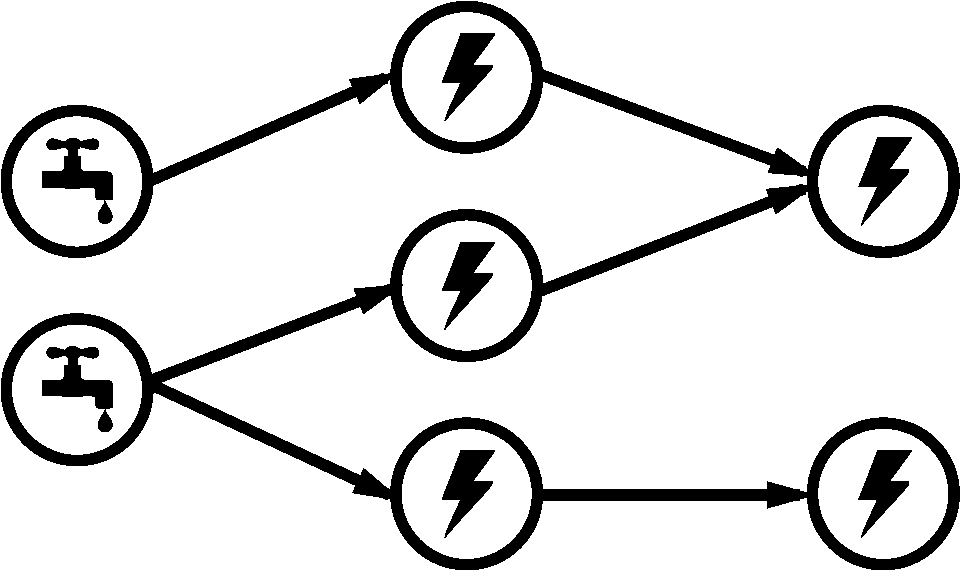
\includegraphics[scale=0.3]{pdf/topology.pdf}
	\caption{An example topology.}
	\label{fig:topology}
\end{figure}

\section{Additional Concepts}

\begin{description}
  \item[Stream] A stream is defined as an unbounded sequence of tuples. Streams can be thought of as edges connecting bolts and spouts (vertices) of a topology
  \item[Tuple] A tuple wraps named fields and their values. The values of fields can be of different types. When a component emits a tuple to a stream it sends that tuple to every bolt subscribed to the stream.
  \item[Stream Grouping] Every bolt needs to have a type of stream grouping associated with it. This grouping decides the means of distributing the tuples coming from its input streams amongst the instances of the bolt task.
  	  \todo{Maybe list Grouping types} 
\end{description}

All the components of a Storm topology execute in parallel. A user can specify how much parallelism he wants associated with every component and Storm spawns the necessary number of threads.

\section{Example Topology}

\todo{Maybe write a few paragraphs about some sample topology}

\section{Storm Architecture}

\todo{Maybe highlight similarities to Hadoop}

A Storm cluster adopts a Master-Worker pattern. To set up a Storm topology, user launches daemon processes on nodes of the cluster and submits the topology to the master node. The worker nodes receive task assignments from the master and execute on them.

\subsection{Master (Nimbus) Node}

The master node runs a server daemon called Nimbus. The main role of Nimbus is to receive topology submissions from clients. Upon receiving a topology submission, Nimbus takes the following steps:

\todo{Is listing the steps involved the right way to explain it?}

\begin{enumerate}
	\item Validates the topology.
	\item Distributes the topology source code across the cluster.
	\item Runs the scheduler and makes worker assignments.
	\item Activates the topology.
\end{enumerate}

\todo{Link to Apache Thrift here?}
Nimbus is an Apache Thrift service (more on Thrift in section \ref{sec:serialisation}) that listens to commands submitted by clients and modifies the state of a cluster accordingly. Following are commands supported by Nimbus:

\todo{Is listing this really necessary?}

\begin{description}
	\item[Submit a topology] \hfill \\
	Clients can submit a topology defined in a jar file. The Nimbus service then ensures that the topology configuration and resources are distributed across the cluster and starts executing the topology.
	\item[Kill a topology] \hfill \\
	Nimbus can stop running a topology and remove it from the cluster. The cluster can continue executing other topologies.
	\item[Activate/deactivate a topology] \hfill \\
	Topologies can be deactivated and reactivated by Nimbus.
	\item[Rebalance a topology] \hfill \\
	Nimbus can rebalance a topology across more nodes. Thus if the number of nodes in the cluster changes the user can increase or decrease the number of nodes involved in the topology.
\end{description}


\subsection{Worker Nodes}

The worker nodes run a daemon called Supervisor. This daemon launches worker processes which execute the tasks assigned to the node. A worker node runs the following processes:

\begin{description}
	\item[Supervisor] \hfill \\
	A supervisor is a daemon process, ran under supervision, that launches worker processes. This daemon is what the user runs on a worker node to make it part of the cluster. It launches worker processes and assigns them a port they can listen on.
	\item[Worker] \hfill \\
	A worker process is assigned a port and listens to tuple messages on a socket associated with the port. A worker launches executor threads as required by the topology. Whenever it receives a tuple, it puts it on a queue where it is picked up by one or more executors of the worker process. Furthermore, the worker has a transfer queue where worker's executors enqueue tuples ready to be sent down the stream.
	\item[Executor] \hfill \\
	An executor controls the parallelism within a worker process. Every executor runs in a separate thread. An executor's job is to pick up tuples from the receiver queue, perform the task of a component it represents, and put the transformed tuples on the transfer queue of its worker. Within its thread, executor runs one (the usual case) or more tasks.
	\item[Task] \hfill \\
	A task performs the actual data processing. However, within an executor thread all the tasks are executed sequentially. The main reason for having tasks is that the number of tasks stays the same throughout the lifetime of a topology but the number of executors can change (by rebalancing). Thus if some worker nodes in the cluster go down, the topology can continue executing with the same number of tasks as before.
\end{description}

\subsection{Zookeeper Nodes}

Lastly, the cluster contains a number of Zookeeper nodes which coordinate the communication between the master and the workers. The Zookeeper nodes can be thought of as the glue of the network. They ensure that messages are delivered.

\section{Serialisation}
\label{sec:serialisation}

Since Storm topologies execute on a cluster all the components need to be serialisable. This is achieved with Apache Thrift. Components are defined as Thrift objects and Thrift generates all the Java serialisation code automatically.

Furthermore, since Nimbus is a Thrift service Thrift generates all the code required for RPC support. This allows for easy cross-language communication.


%%%%%%%%%%%%%%%%%%%%%%%%%%%%%%%%%%%%%%%%%%%%%
%%
%%				   DESIGN
%%
%%%%%%%%%%%%%%%%%%%%%%%%%%%%%%%%%%%%%%%%%%%%%


\chapter{Bringing Storm to Multi-core}

% - Explain why original Storm is bad
% - Explain high-level
% - Explain Nimbus - assignments are useless though
% - Explain how executors interact within a worker - messages


The design of Storm-MC was ported over from Apache Storm. This enabled rapid progress while guaranteeing compatibility with Apache Storm API. Clearly, however, some differences had to be made to take advantage of a multi-core machine performance. This chapter explains the design of Storm-MC.

\section{Apache Storm on Multi-core}

To begin, we discuss why Apache Storm does not perform well on a single machine. Storm can be ran in local mode where it only simulates execution on a cluster. This mode was created for being able to develop and debug topologies without needing access to a cluster. There are several reasons why the local mode is not as performant as it could be.

\begin{description}
	\item[Multi-process Nature of Storm] \hfill \\
	In general, multi-process applications suffer overhead from inter-process communication and are generally slower than their multi-threaded counterparts \cite{Kumar:2013:HSD:2536274.2536314}.
	\item[Fault Tolerance] \hfill \\
	Storm is made to be fault-tolerant. This means that it can guarantee a tuple being processed from its spout all the way to its final bolt. To do this it adds an additional acker bolt to every topology. This bolt acts as a root of a tree with the nodes being all the components the tuple "goes" through. If the tuple gets successfully processed by a component its node is marked as "acked". Hence once all nodes of the tree are marked as "acked" Storm can guarantee the tuple was processed.
	\todo{Change "goes" and "acked" to something else.}
	\item[Redundant threads] \hfill \\
	Storm runs many threads which are only useful in distributed context. Indeed, during our experiments we found that a topology with 8 executors was being executed with 64 threads. This included threads which were used as timeout timers or to send heartbeats and were unnecessary in a multi-core setting. Obviously, not all of them were executing in parallel but there is clearly room for reduction.
	\todo{Maybe include Thread Dump and a graph of thread counts}
\end{description}

\section{Storm-MC Architecture}

\begin{figure}[!htb]
	\centering
	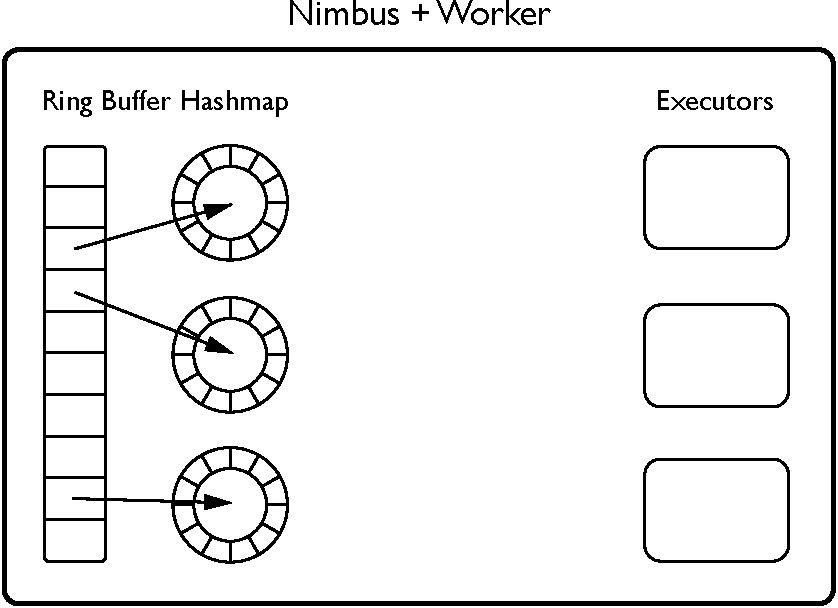
\includegraphics[scale=0.7]{pdf/storm_mc_arch.pdf}
	\caption{Storm-MC Architecture.}
	\label{fig:architecture}
\end{figure}

The overall architecture of Storm-MC can be seen in figure \ref{fig:architecture}. The design we adopted for porting worker nodes is to only have one worker process running multiple executor threads. Additionally, the code for the Nimbus daemon was merged with the worker. This design has several benefits:

\begin{itemize}
	\item All the inter-thread communication is occurring within one Worker.
	\item Supervisor can be removed as there is no need to synchronise workers.
	\item There is no need to simulate over-the-network message passing.
	\item Message passing between executor threads within a worker stays the same.
\end{itemize}

\subsection{Nimbus}

\todo{Rewrite paragraph below, too informal.}
In Apache Storm, Nimbus runs as a server that communicates with possibly multiple clients. While appropriate for a system running on a cluster this is unnecessary on a single machine. Thus to run a topology on Storm-MC one only has to import the library into their project and use it as a standard Java library. To kill the topology, one only needs to send the kill signal as in a standard Java program. Furthermore, there is no need for activating and deactivating as the user can just kill and resubmit the topology. Lastly, rebalancing does not really transfer to a multi-core system and was thusly omitted.

As can be understood from the previous paragraph, Storm-MC does not support running multiple topologies at the same time. However, to do that one only needs to run a separate process. This is because unlike on the cluster different topologies do not need to share any memory and it is more natural to execute them as separate processes.
\todo{Mention things like cache lines in support of above argument.}

Additionally, Storm-MC does not support any scheduling. Since there is only one topology running at a time and the hardware configuration of the machine does not change, the parallelism is clearly defined by the number of executors per component specified in the topology configuration.

In light of this Storm-MC is (almost) completely stateless. The state that was managed by Zookeeper in Apache Storm was completely stripped away.

\subsection{Worker}

\subsection{Message Exchange}

LMAX Disruptor is used for tuple passing between components of a stream. Detailed background of how Disruptor works and its performance benchmarks can be found in \cite{Thompson_Farley_Barker_Gee_Stewart_2011}.

There were two types of tuple transfers in Apache Storm:

\begin{description}
	\item[Inter-worker (remote) transfers] \hfill \\
	When the tuple is sent to a different worker, it is put on a disruptor buffer by an executor thread and picked up by a separate sender thread which sends it across the network to the executors subscribed to the stream. The worker of these executors runs a receiver thread which listens to messages on its port and puts the tuples on disruptor buffers of the corresponding executors.
	\item[Intra-worker (local) transfers] \hfill \\
	When the tuple is sent within the same worker, it is put directly on the disruptor buffer of the executor thus avoiding sending a network message to the same machine.
\end{description}

Since Storm-MC only has one worker process, all tuple transfers are local. Thus, a map of executor identifier to disruptor buffers is maintained. Hence, an executor thread picks up a tuple from the ring buffer corresponding to its identifier and after processing the tuple inserts it into a buffer of executors subscribed to its output stream.

\section{Things Not Included in Storm-MC}

\todo{This section name should be rephrased.}
\todo{Maybe present this as a table of features.}

%%%%%%%%%%%%%%%%%%%%%%%%%%%%%%%%%%%%%%%%%%%%%
%%
%%				   EVALUATION
%%
%%%%%%%%%%%%%%%%%%%%%%%%%%%%%%%%%%%%%%%%%%%%%


\chapter{Evaluation}

\section{Performance}


%%%%%%%%%%%%%%%%%%%%%%%%%%%%%%%%%%%%%%%%%%%%%
%%
%%				CONCLUSION
%%
%%%%%%%%%%%%%%%%%%%%%%%%%%%%%%%%%%%%%%%%%%%%%


\chapter{Conclusion}

\section{Future Work}


% use the following and \cite{} as above if you use BibTeX
% otherwise generate bibtem entries
\bibliographystyle{plain}
\bibliography{mybibfile}

\end{document}
